\documentclass[12pt, a4paper]{extarticle}
\usepackage{GOST}

\makeatletter
\renewcommand\@biblabel[1]{#1.}
\makeatother


\graphicspath{{images/}}

\begin{document}
\begin{table}[ht]
	\centering
	\begin{tabular}{|c|p{400pt}|} 
	\hline
		\begin{tabular}[c]{@{}c@{}} 
\includegraphics[scale=0.8]{b_logo} \\\end{tabular} &
		\footnotesize\begin{tabular}[c]{@{}c@{}}\textbf{Министерство~науки~и~высшего~образования~Российской~Федерации}\\\textbf{Федеральное~государственное~бюджетное~образовательное~учреждение}\\\textbf{~высшего~образования}\\\textbf{«Московский~государственный~технический~университет}\\\textbf{имени~Н.Э.~Баумана}\\\textbf{(национальный~исследовательский~университет)»}\\\textbf{(МГТУ~им.~Н.Э.~Баумана)}\\\end{tabular}  \\
	\hline
	\end{tabular}
\end{table}
\noindent\rule{\textwidth}{4pt}
\noindent\rule[14pt]{\textwidth}{1pt}
\hfill 
\noindent
\makebox{ФАКУЛЬТЕТ~}%
\makebox[\textwidth][l]{\underline{~~~~~«Информатика и системы управления»~~~~~~~~~~~~~~~~~~~~~~~~~}}%
\\
\noindent
\makebox{КАФЕДРА~}%
\makebox[\textwidth][l]{\underline{«Программное обеспечение ЭВМ и информационные технологии»}}%

\begin{center}
	\vspace{1.5cm}
	{\bf\huge Расчетно-пояснительная записка\par}
	{\bf\Large к курсовой работе\par}
	\vspace{0cm}
\end{center}


\noindent
\makebox{\large{\bf Тема:}~~~}
\makebox[\textwidth][l]{\large\underline{~Разработка протокола с дедупликацией~~~~~~~~~~~~~}}\\

\noindent
\makebox{\large{\bf Дисциплина:}~~~}
\makebox[\textwidth][l]{\large\underline{~Компьютерные сети~~~~~~~~~~~~~~~~~~~~}}\\

\vspace{1cm}
\noindent
\begin{tabular}{l c c c c c}
    Студент      & ~ИУ7-75Б~       & \hspace{2.5cm} & \hspace{3cm}               & &  П.К Хетагуров \\\cline{2-2}\cline{4-4} \cline{6-6} 
    \hspace{3cm} & {\footnotesize(Группа)} &                & {\footnotesize(Подпись, дата)} & & {\footnotesize(И.О. Фамилия)}
\end{tabular}

\vspace{0.5cm}

\noindent
\begin{tabular}{l c c c c}
    Руководитель проекта & \hspace{3.3cm}   & \hspace{3.5cm}              & & Н.О. Рогозин \\\cline{3-3} \cline{5-5} 
    \hspace{2.9cm}  &              & {\footnotesize(Подпись, дата)} & & {\footnotesize(И.О. Фамилия)}
\end{tabular}

\begin{center}	
	\vfill
	\large \textit {Москва, 2021}
\end{center}

\thispagestyle {empty}
\pagebreak
\section{Задание}

Написать smtp-клиент, который

\begin{enumerate}
\item В качестве входных данных (аргументы командной строки) получает: \\
    адрес получателя, адрес отправителя, пароль.
	\item 
Использует один из открытых smtp-серверов для доставки MIME-сообщений, включая приложения, если они есть, в соответствии с вариантом. \\
Вариант = номер студента по списку в Электронном Университете \% кол-во вариантов.
	\item Дополнительная задача зависит от варианта.

 	\begin{enumerate}
	\item Доставка сообщений выполняется с регулярным интервалом. Интервал и тело сообщения, имя файла для прикрепления (опционально) вводятся с клавиатуры. 
	\item  В качестве дополнительного параметра задается ключевое слово. По данному ключевому слову выполняется поиск в текстовых файлах в папке клиента, При обнаружении слова файл прикрепляется к письму.

	\item Доставка сообщений выполняется в определенное время. Время и тело сообщения, имя файла для прикрепления (опционально) вводятся с клавиатуры. 
	\end{enumerate}
\end{enumerate}
Допускается использование любого ЯП и фреймворков.

\section{Результаты}
Дополнительное задание 1. Доставка сообщений выполняется с регулярным интервалом. Интервал и тело сообщения, имя файла для прикрепления (опционально) вводятся с клавиатуры. 


Так как не нашел соответствие вариантов и SMTP-серверов был выбран SMTP-сервер smtp.yandex.ru.

Для реализации был выбран язык C\#.

Работа программы:
\begin{figure}[H]
	\centering
	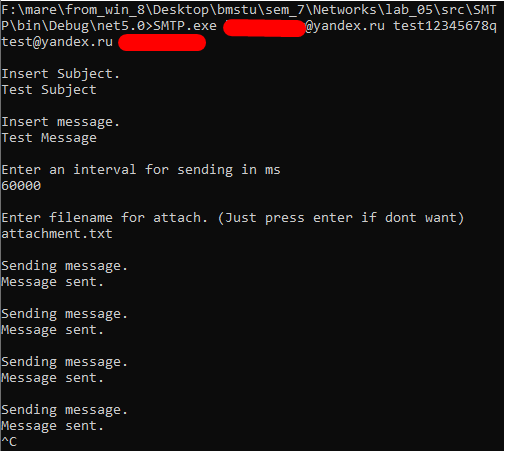
\includegraphics[scale=0.9]{images/work.png}
	\caption{Работа программы}
\end{figure}

В результате начали приходить письма на указанный адрес с интервалос в 60 секунд с заданным телом и прикреплением.

\begin{figure}[H]
	\centering
	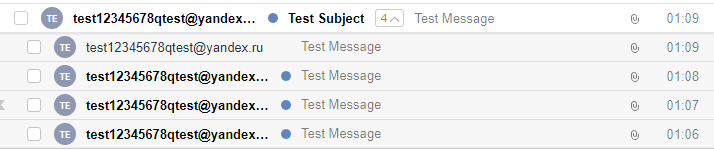
\includegraphics[scale=0.9]{images/res.png}
	\caption{Результат работы программы}
\end{figure}

Отдельное письмо:
\begin{figure}[H]
	\centering
	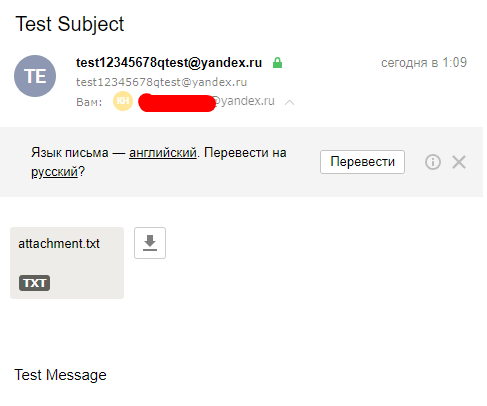
\includegraphics[scale=0.9]{images/resSingle.png}
	\caption{Отдельное письмо}
\end{figure}

\begin{lstlisting}[language={[Sharp]C}, caption={Программа}]
using System;
using System.Net;
using System.Net.Mail;
using System.Net.Mime;
using System.Threading;
using System.ComponentModel;

namespace SMTP
{
    class Program
    {
        const string SERVER = "smtp.yandex.ru";
        const int PORT = 587;
        static void Main(string[] args)
        {
            var receiver = args[0];
            var sender = args[1];
            var pass = args[2];


            SmtpClient client = new SmtpClient(SERVER, PORT);
            MailAddress to = new MailAddress(receiver);
            MailAddress from = new MailAddress(sender);

            client.Credentials = new NetworkCredential(sender, pass);   
            client.EnableSsl = true;

            Console.WriteLine("\nInsert Subject.");
            string message_subject = Console.ReadLine();
            Console.WriteLine("\nInsert message.");
            string message_body = Console.ReadLine();
            Console.WriteLine("\nEnter an interval for sending in ms");
            int interval = 1;
            if (!int.TryParse(Console.ReadLine(), out interval))
            { 
                Console.WriteLine("You have entered an incorrect value.");
                return;
            }
            Console.WriteLine("\nEnter filename for attach. (Just press enter if dont want)");
            string file = Console.ReadLine();

            MailMessage message = new MailMessage(from, to);
            if (file.Length != 0)
            {
                var attachment = new Attachment(file);
                if (attachment != null) {
                    message.Attachments.Add(attachment);
                }
            }

            message.Body = message_body;
            message.Subject = message_subject;

            client.SendCompleted += new SendCompletedEventHandler(SendCompletedCallback);

            while (true) {
                client.SendAsync(message, "test");
                Console.WriteLine("\nSending message.");
                Thread.Sleep(interval);
            }
        }

        private static void SendCompletedCallback(object sender, AsyncCompletedEventArgs e)
        {
            if (e.Cancelled)
            {
                Console.WriteLine("Send canceled.");
            }
            if (e.Error != null)
            {
                Console.WriteLine("{0}", e.Error.ToString());
            }
            else
            {
                Console.WriteLine("Message sent.");
            }
        }
    }
}

\end{lstlisting}

\end{document}




